\documentclass[UTF8,11pt]{ctexart}
\usepackage[a4paper,margin=22mm]{geometry}
\usepackage{graphicx,enumitem,amssymb,tabularx}
\usepackage[normalem]{ulem}
\usepackage{xeCJKfntef}
\setlength{\parindent}{0pt}
\setlength{\parskip}{.6em}
\sloppy
\begin{document}
\section*{2000年考研英语（统一卷）}
\subsection*{2000 年全国硕士研究生招生考试英语试题}


\subsection*{\textbf{Section I Use of English}}


\subsection*{\textbf{Directions:}}


For each numbered blank in the following passage, there are four choices marked A, B, C and D. Choose the best one and mark your answer on ANSWER SHEET 1 by blackening the corresponding letter in the brackets with a pencil. (10 points)


If a farmer wishes to succeed, he must try to keep a wide gap between his consumption and his production. He must store a large quantity of grain \uline{1} consuming all his grain immediately. He can continue to support himself and his family \uline{2} he produces a surplus. He must use this surplus in three ways: as seed for sowing, as an insurance \uline{3} the unpredictable effects of bad weather and as a commodity which he must sell in order to \uline{4} old agricultural implements and obtain chemical fertilizers to \uline{5} the soil. He may also need money to construct irrigation \uline{6} and improve his farm in other ways. If no surplus is available, a farmer cannot be \uline{7 }. He must either sell some of his property or \uline{8} extra funds in the form of loans. Naturally he will try to borrow money at a low \uline{9} of interest, but loans of this kind are not \uline{10} obtainable.


\noindent\begin{tabularx}{\linewidth}{@{}lXXXX@{}}1. & \textbf{A.} other than & \textbf{B.} as well as & \textbf{C.} instead of & \textbf{D.} more than\\\end{tabularx}\par

\noindent\begin{tabularx}{\linewidth}{@{}lXXXX@{}}2. & \textbf{A.} only if & \textbf{B.} much as & \textbf{C.} long before & \textbf{D.} ever since\\\end{tabularx}\par

\noindent\begin{tabularx}{\linewidth}{@{}lXXXX@{}}3. & \textbf{A.} for & \textbf{B.} against & \textbf{C.} of & \textbf{D.} towards\\\end{tabularx}\par

\noindent\begin{tabularx}{\linewidth}{@{}lXXXX@{}}4. & \textbf{A.} replace & \textbf{B.} purchase & \textbf{C.} supplement & \textbf{D.} dispose\\\end{tabularx}\par

\noindent\begin{tabularx}{\linewidth}{@{}lXXXX@{}}5. & \textbf{A.} enhance & \textbf{B.} mix & \textbf{C.} feed & \textbf{D.} raise\\\end{tabularx}\par

\noindent\begin{tabularx}{\linewidth}{@{}lXXXX@{}}6. & \textbf{A.} vessels & \textbf{B.} routes & \textbf{C.} paths & \textbf{D.} channels\\\end{tabularx}\par

\noindent\begin{tabularx}{\linewidth}{@{}lXXXX@{}}7. & \textbf{A.} self-confident & \textbf{B.} self-sufficient & \textbf{C.} self-satisfied & \textbf{D.} self-restrained\\\end{tabularx}\par

\noindent\begin{tabularx}{\linewidth}{@{}lXXXX@{}}8. & \textbf{A.} search & \textbf{B.} save & \textbf{C.} offer & \textbf{D.} seek\\\end{tabularx}\par

\noindent\begin{tabularx}{\linewidth}{@{}lXXXX@{}}9. & \textbf{A.} proportion & \textbf{B.} percentage & \textbf{C.} rate & \textbf{D.} ratio\\\end{tabularx}\par

\noindent\begin{tabularx}{\linewidth}{@{}lXXXX@{}}10. & \textbf{A.} genuinely & \textbf{B.} obviously & \textbf{C.} presumably & \textbf{D.} frequently\\\end{tabularx}\par

\subsection*{\textbf{Section II Reading Comprehension}}


\subsection*{\textbf{Part A}}


\subsection*{\textbf{Directions:}}


Each of the passages below is followed by some questions. For each question there are four answers marked A, B, C and D. Read the passages carefully and choose the best answer to each of the questions. Then mark your answer on ANSWER SHEET 1 by blackening the corresponding letter in the brackets with a pencil. (40 points)


\subsection*{\textbf{Text 1}}


A history of long and effortless success can be a dreadful handicap, but, if properly handled, it may become a driving force. When the United States entered just such a glowing period after the end of the Second World War, it had a market eight times larger than any competitor, giving its industries unparalleled economies of scale. Its scientists were the world’s best; its workers the most skilled. America and Americans were prosperous beyond the dreams of the Europeans and Asians whose economies the war had destroyed.


It was inevitable that this primacy should have narrowed as other countries grew richer. Just as inevitably, the retreat from predominance proved painful. By the mid-1980s Americans had found themselves at a loss over their fading industrial competitiveness. Some huge American industries, such as consumer electronics, had shrunk or vanished in the face of foreign competition. By 1987 there was only one American television maker left, Zenith. (Now there is none: Zenith was bought by South Korea’s LG Electronics in July.) Foreign-made cars and textiles were sweeping into the domestic market. America’s machine-tool industry was on the ropes. For a while it looked as though the making of semiconductors, which America had invented and which sat at the heart of the new computer age, was going to be the next casualty.


All of this caused a crisis of confidence. Americans stopped taking prosperity for granted. They began to believe that their way of doing business was failing, and that their incomes would therefore shortly begin to fall as well. The mid-1980s brought one inquiry after another into the causes of America’s industrial decline. Their sometimes sensational findings were filled with warnings about the growing competition from overseas.


How things have changed! In 1995 the United States can look back on five years of solid growth while Japan has been struggling. Few Americans attribute this solely to such obvious causes as a devalued dollar or the turning of the business cycle. Self-doubt has yielded to blind pride. “American industry has changed its structure, has gone on a diet, has learnt to be more quick-witted,” according to Richard Cavanagh, executive dean of Harvard’s Kennedy School of Government. “It makes me proud to be an American just to see how our businesses are improving their productivity,” says Stephen Moore of the Cato Institute, a think-tank in Washington, DC. And William Sahlman of the Harvard Business School believes that people will look back on this period as “a golden age of business management in the United States.”


11. The U.S. achieved its predominance after World War II because \_\_\_\_\_\_


\begin{itemize}[leftmargin=2em,itemsep=.2em,topsep=.4em]\item[A.] it had made painstaking efforts towards this goal.
\item[B.] its domestic market was eight times larger than before.
\item[C.] the war had destroyed the economies of most potential competitors.
\item[D.] the unparalleled size of its workforce had given an impetus to its economy.
\end{itemize}

12. The loss of U.S. predominance in the world economy in the 1980s is manifested in the


fact that the American \_\_\_\_\_\_


\begin{itemize}[leftmargin=2em,itemsep=.2em,topsep=.4em]\item[A.] TV industry had withdrawn to its domestic market.
\item[B.] semiconductor industry had been taken over by foreign enterprises.
\item[C.] machine-tool industry had collapsed after suicidal actions.
\item[D.] auto industry had lost part of its domestic market.
\end{itemize}

13. What can be inferred from the passage?


\begin{itemize}[leftmargin=2em,itemsep=.2em,topsep=.4em]\item[A.] It is human nature to shift between self-doubt and blind pride.
\item[B.] Intense competition may contribute to economic progress.
\item[C.] The revival of the economy depends on international cooperation.
\item[D.] A long history of success may pave the way for further development.
\end{itemize}

14. The author seems to believe the revival of the U.S. economy in the 1990s can be


attributed to the \_\_\_\_\_\_


\begin{itemize}[leftmargin=2em,itemsep=.2em,topsep=.4em]\item[A.] turning of the business cycle.
\item[B.] restructuring of industry.
\item[C.] improved business management.
\item[D.] success in education.
\end{itemize}

\subsection*{\textbf{Text 2}}


Being a man has always been dangerous. There are about 105 males born for every 100 females, but this ratio drops to near balance at the age of maturity, and among 70-year-olds there are twice as many women as men. But the great universal of male mortality is being changed. Now, boy babies survive almost as well as girls do. This means that, for the first time, there will be an excess of boys in those crucial years when they are searching for a mate. More important, another chance for natural selection has been removed. Fifty years ago, the chance of a baby (particularly a boy baby) surviving depended on its weight. A kilogram too light or too heavy meant almost certain death. Today it makes almost no difference. Since much of the variation is due to genes, one more agent of evolution has gone.


There is another way to commit evolutionary suicide: stay alive, but have fewer children. Few people are as fertile as in the past. Except in some religious communities, very few women have 15 children. Nowadays the number of births, like the age of death, has become average. Most of us have roughly the same number of offspring. Again, differences between people and the opportunity for natural selection to take advantage of it have diminished. India shows what is happening. The country offers wealth for a few in the great cities and poverty for the remaining tribal peoples. The grand mediocrity of today — everyone being the same in survival and number of offspring — means that natural selection has lost 80\% of its power in upper-middle-class India compared to the tribes.


For us, this means that evolution is over; the biological Utopia has arrived. Strangely, it has involved little physical change. No other species fills so many places in nature. But in the past 100,000 years — even the past 100 years — our lives have been transformed but our bodies have not. We did not evolve, because machines and society did it for us. Darwin had a phrase to describe those ignorant of evolution: they “look at an organic being as a savage looks at a ship, as at something wholly beyond his comprehension.” No doubt we will remember a 20th century way of life beyond comprehension for its ugliness. But however amazed our descendants may be at how far from Utopia we were, they will look just like us.


15. What used to be the danger in being a man according to the first paragraph?


\begin{itemize}[leftmargin=2em,itemsep=.2em,topsep=.4em]\item[A.] A lack of mates.
\item[B.] A fierce competition.
\item[C.] A lower survival rate.
\item[D.] A defective gene.
\end{itemize}

16. What does the example of India illustrate?


\begin{itemize}[leftmargin=2em,itemsep=.2em,topsep=.4em]\item[A.] Wealthy people tend to have fewer children than poor people.
\item[B.] Natural selection hardly works among the rich and the poor.
\item[C.] The middle class population is 80\% smaller than that of the tribes.
\item[D.] India is one of the countries with a very high birth rate.
\end{itemize}

17. The author argues that our bodies have stopped evolving because \_\_\_\_\_\_


\begin{itemize}[leftmargin=2em,itemsep=.2em,topsep=.4em]\item[A.] life has been improved by technological advance.
\item[B.] the number of female babies has been declining.
\item[C.] our species has reached the highest stage of evolution.
\item[D.] the difference between wealth and poverty is disappearing.
\end{itemize}

18. Which of the following would be the best title for the passage?


\begin{itemize}[leftmargin=2em,itemsep=.2em,topsep=.4em]\item[A.] Sex Ratio Changes in Human Evolution.
\item[B.] Ways of Continuing Man’s Evolution.
\item[C.] The Evolutionary Future of Nature.
\item[D.] Human Evolution Going Nowhere.
\end{itemize}

\subsection*{\textbf{Text 3}}


When a new movement in art attains a certain fashion, it is advisable to find out what its advocates are aiming at, for, however farfetched and unreasonable their principles may seem today, it is possible that in years to come they may be regarded as normal. With regard to Futurist poetry, however, the case is rather difficult, for whatever Futurist poetry may be — even admitting that the theory on which it is based may be right — it can hardly be classed as Literature.


This, in brief, is what the Futurist says: for a century, past conditions of life have been conditionally speeding up, till now we live in a world of noise and violence and speed. Consequently, our feelings, thoughts and emotions have undergone a corresponding change. This speeding up of life, says the Futurist, requires a new form of expression. We must speed up our literature too, if we want to interpret modern stress. We must pour out a large stream of essential words, unhampered by stops, or qualifying adjectives, or finite verbs. Instead of describing sounds we must make up words that imitate them; we must use many sizes of type and different colored inks on the same page, and shorten or lengthen words at will.


Certainly their descriptions of battles are confused. But it is a little upsetting to read in the explanatory notes that a certain line describes a fight between a Turkish and a Bulgarian officer on a bridge off which they both fall into the river — and then to find that the line consists of the noise of their falling and the weights of the officers: “Pluff! Pluff! A hundred and eighty-five kilograms.”


This, though it fulfills the laws and requirements of Futurist poetry, can hardly be classed as Literature. All the same, no thinking man can refuse to accept their first proposition: that a great change in our emotional life calls for a change of expression. The whole question is really this: have we essentially changed?


19. This passage is mainly \_\_\_\_\_\_


\begin{itemize}[leftmargin=2em,itemsep=.2em,topsep=.4em]\item[A.] a survey of new approaches to art.
\item[B.] a review of Futurist poetry.
\item[C.] about merits of the Futurist movement.
\item[D.] about laws and requirements of literature.
\end{itemize}

20. When a novel literary idea appears, people should try to \_\_\_\_\_\_


\begin{itemize}[leftmargin=2em,itemsep=.2em,topsep=.4em]\item[A.] determine its purposes.
\item[B.] ignore its flaws.
\item[C.] follow the new fashions.
\item[D.] accept the principles.
\end{itemize}

21. Futurists claim that we must \_\_\_\_\_\_


\begin{itemize}[leftmargin=2em,itemsep=.2em,topsep=.4em]\item[A.] increase the production of literature.
\item[B.] use poetry to relieve modern stress.
\item[C.] develop new modes of expression.
\item[D.] avoid using adjectives and verbs.
\end{itemize}

22. The author believes that Futurist poetry is \_\_\_\_\_\_


\begin{itemize}[leftmargin=2em,itemsep=.2em,topsep=.4em]\item[A.] based on reasonable principles.
\item[B.] new and acceptable to ordinary people.
\item[C.] indicative of a basic change in human nature.
\item[D.] more of a transient phenomenon than literature.
\end{itemize}

\subsection*{\textbf{Text 4}}


Aimlessness has hardly been typical of the postwar Japan whose productivity and social harmony are the envy of the United States and Europe. But increasingly the Japanese are seeing a decline of the traditional work-moral values. Ten years ago young people were hardworking and saw their jobs as their primary reason for being, but now Japan has largely fulfilled its economic needs, and young people don’t know where they should go next.


The coming of age of the postwar baby boom and an entry of women into the male-dominated job market have limited the opportunities of teen-agers who are already questioning the heavy personal sacrifices involved in climbing Japan’s rigid social ladder to good schools and jobs. In a recent survey, it was found that only 24.5 percent of Japanese students were fully satisfied with school life, compared with 67.2 percent of students in the United States. In addition, far more Japanese workers expressed dissatisfaction with their jobs than did their counterparts in the 10 other countries surveyed.


While often praised by foreigners for its emphasis on the basics, Japanese education tends to stress test taking and mechanical learning over creativity and self-expression. “Those things that do not show up in the test scores — personality, ability, courage or humanity — are completely ignored,” says Toshiki Kaifu, chairman of the ruling Liberal Democratic Party’s education committee. “Frustration against this kind of thing leads kids to drop out and run wild.” Last year Japan experienced 2,125 incidents of school violence, including 929 assaults on teachers. Amid the outcry, many conservative leaders are seeking a return to the prewar emphasis on moral education. Last year Mitsuo Setoyama, who was then education minister, raised eyebrows when he argued that liberal reforms introduced by the American occupation authorities after World War II had weakened the “Japanese morality of respect for parents.”


But that may have more to do with Japanese life-styles. “In Japan,” says educator Yoko Muro, “it’s never a question of whether you enjoy your job and your life, but only how much you can endure.” With economic growth has come centralization; fully 76 percent of Japan’s 119 million citizens live in cities where community and the extended family have been abandoned in favor of isolated, two-generation households. Urban Japanese have long endured lengthy commutes (travels to and from work) and crowded living conditions, but as the old group and family values weaken, the discomfort is beginning to tell. In the past decade, the Japanese divorce rate, while still well below that of the United States, has increased by more than 50 percent, and suicides have increased by nearly one-quarter.


23. In the Westerners’ eyes, the postwar Japan was \_\_\_\_\_\_


\begin{itemize}[leftmargin=2em,itemsep=.2em,topsep=.4em]\item[A.] under aimless development.
\item[B.] a positive example.
\item[C.] a rival to the West.
\item[D.] on the decline.
\end{itemize}

24. According to the author, what may chiefly be responsible for the moral decline of


Japanese society?


\begin{itemize}[leftmargin=2em,itemsep=.2em,topsep=.4em]\item[A.] Women’s participation in social activities is limited.
\item[B.] More workers are dissatisfied with their jobs.
\item[C.] Excessive emphasis has been placed on the basics.
\item[D.] The life-style has been influenced by Western values.
\end{itemize}

25. Which of the following is true according to the author?


\begin{itemize}[leftmargin=2em,itemsep=.2em,topsep=.4em]\item[A.] Japanese education is praised for helping the young climb the social ladder.
\item[B.] Japanese education is characterized by mechanical learning as well as creativity.
\item[C.] More stress should be placed on the cultivation of creativity.
\item[D.] Dropping out leads to frustration against test taking.
\end{itemize}

26. The change in Japanese life-style is revealed in the fact that \_\_\_\_\_\_


\begin{itemize}[leftmargin=2em,itemsep=.2em,topsep=.4em]\item[A.] the young are less tolerant of discomforts in life.
\item[B.] the divorce rate in Japan exceeds that in the U.S.
\item[C.] the Japanese endure more than ever before.
\item[D.] the Japanese appreciate their present life.
\end{itemize}

\subsection*{\textbf{Text 5}}


If ambition is to be well regarded, the rewards of ambition — wealth, distinction, control over one’s destiny — must be deemed worthy of the sacrifices made on ambition’s behalf. If the tradition of ambition is to have vitality, it must be widely shared; and it especially must be highly regarded by people who are themselves admired, the educated not least among them. In an odd way, however, it is the educated who have claimed to have given up on ambition as an ideal. What is odd is that they have perhaps most benefited from ambition — if not always their own then that of their parents and grandparents. There is a heavy note of hypocrisy in this, a case of closing the barn door after the horses have escaped — with the educated themselves riding on them.


Certainly people do not seem less interested in success and its signs now than formerly. Summer homes, European travel, BMWs — the locations, place names and name brands may change, but such items do not seem less in demand today than a decade or two years ago. What has happened is that people cannot confess fully to their dreams, as easily and openly as once they could, lest they be thought pushing, acquisitive and vulgar. Instead, we are treated to fine hypocritical spectacles, which now more than ever seem in ample supply: the critic of American materialism with a Southampton summer home; the publisher of radical books who takes his meals in three-star restaurants; the journalist advocating participatory democracy in all phases of life, whose own children are enrolled in private schools. For such people and many more perhaps not so exceptional, the proper formulation is, “Succeed at all costs but avoid appearing ambitious.”


The attacks on ambition are many and come from various angles; its public defenders are few and unimpressive, where they are not extremely unattractive. As a result, the support for ambition as a healthy impulse, a quality to be admired and fixed in the mind of the young, is probably lower than it has ever been in the United States. This does not mean that ambition is at an end, that people no longer feel its stirrings and promptings, but only that, no longer openly honored, it is less openly professed. Consequences follow from this, of course, some of which are that ambition is driven underground, or made sly. Such, then, is the way things stand: on the left angry critics, on the right stupid supporters, and in the middle, as usual, the majority of earnest people trying to get on in life.


27. It is generally believed that ambition may be well regarded if \_\_\_\_\_\_


\begin{itemize}[leftmargin=2em,itemsep=.2em,topsep=.4em]\item[A.] its returns well compensate for the sacrifices.
\item[B.] it is rewarded with money, fame and power.
\item[C.] its goals are spiritual rather than material.
\item[D.] it is shared by the rich and the famous.
\end{itemize}

28. The last sentence of the first paragraph most probably implies that it is \_\_\_\_\_\_


\begin{itemize}[leftmargin=2em,itemsep=.2em,topsep=.4em]\item[A.] customary of the educated to discard ambition in words.
\item[B.] too late to check ambition once it has been let out.
\item[C.] dishonest to deny ambition after the fulfillment of the goal.
\item[D.] impractical for the educated to enjoy benefits from ambition.
\end{itemize}

29. Some people do not openly admit they have ambition because \_\_\_\_\_\_


\begin{itemize}[leftmargin=2em,itemsep=.2em,topsep=.4em]\item[A.] they think of it as immoral.
\item[B.] their pursuits are not fame or wealth.
\item[C.] ambition is not closely related to material benefits.
\item[D.] they do not want to appear greedy and contemptible.
\end{itemize}

30. From the last paragraph the conclusion can be drawn that ambition should be


maintained \_\_\_\_\_\_


\begin{itemize}[leftmargin=2em,itemsep=.2em,topsep=.4em]\item[A.] secretly and vigorously.
\item[B.] openly and enthusiastically.
\item[C.] easily and momentarily.
\item[D.] verbally and spiritually.
\end{itemize}

\subsection*{\textbf{Part B}}


\subsection*{\textbf{Directions:}}


Read the following passage carefully and then translate the underlined segments into Chinese. Your translation must be written clearly on ANSWER SHEET 2. (15 points)


Governments throughout the world act on the assumption that the welfare of their people depends largely on the economic strength and wealth of the community. (31) \uline{Under} \uline{modern conditions, this requires varying measures of centralized control and hence the help} \uline{of} \uline{specialized} \uline{scientists} \uline{such} \uline{as} \uline{economists} \uline{and} \uline{operational} \uline{research} \uline{experts.} (32) \uline{Furthermore, it is obvious that the strength of a country’s economy is directly bound up with} \uline{the efficiency of its agriculture and industry, and that this in turn rests upon the efforts of} \uline{scientists and technologists of all kinds. }It also means that governments are increasingly compelled to interfere in these sectors in order to step up production and ensure that it is utilized to the best advantage. For example, they may encourage research in various ways, including the setting up of their own research centers; they may alter the structure of education, or interfere in order to reduce the wastage of natural resources or tap resources hitherto unexploited; or they may cooperate directly in the growing number of international projects related to science, economics and industry. In any case, all such interventions are heavily dependent on scientific advice and also scientific and technological manpower of all kinds.


(33) \uline{Owing} \uline{to} \uline{the} \uline{remarkable} \uline{development} \uline{in} \uline{mass-communications,} \uline{people} \uline{everywhere are feeling new wants and are being exposed to new customs and ideas, while} \uline{governments are often forced to introduce still further innovations for the reasons given} \uline{above. }At the same time, the normal rate of social change throughout the world is taking place at a vastly accelerated speed compared with the past. For example, (34) \uline{in the early} \uline{industrialized countries of Europe the process of industrialization — with all the far-reaching} \uline{changes in social patterns that followed — was spread over nearly a century, whereas} \uline{nowadays a developing nation may undergo the same process in a decade or so. }All this has the effect of building up unusual pressures and tensions within the community and consequently presents serious problems for the governments concerned. (35) \uline{Additional} \uline{social stresses may also occur because of the population explosion or problems arising from} \uline{mass migration movements — themselves made relatively easy nowadays by modern means} \uline{of transport.} As a result of all these factors, governments are becoming increasingly dependent on biologists and social scientists for planning the appropriate programs and putting them into effect.


\subsection*{\textbf{Section III Writing}}


\textbf{36. Directions:}


\begin{itemize}[leftmargin=2em,itemsep=.2em,topsep=.4em]\item[A.] Study the following two pictures carefully and write an essay of at least 150 words.
\item[B.] Your essay must be written neatly on ANSWER SHEET 2.
\item[C.] Your essay should meet the requirements below:
\end{itemize}

1) Describe the pictures.


2) Deduce the purpose of the drawer of the pictures.


3) Suggest counter-measures.


\begin{center}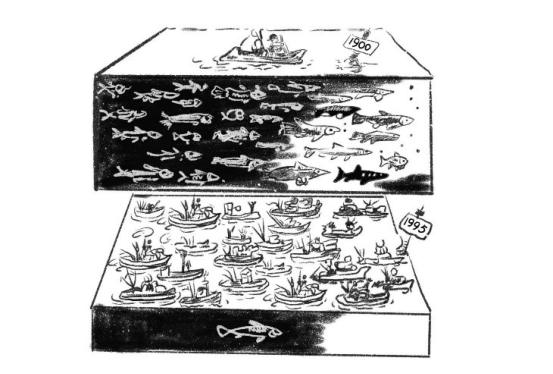
\includegraphics[width=.85\linewidth,height=.55\textheight,keepaspectratio]{2000-01.assets/figure-013-006.png}\end{center}

\begin{center}A Brief History of World Commercial Fishing\end{center}
\end{document}